\documentclass[
ngerman,
toc=listof,
toc=bibliography,
footnotes=multiple,
parskip=half,
numbers=noendperiod
]{scrartcl}
\pdfminorversion=5
\usepackage[utf8]{inputenc}

% !TEX root = document.tex

\newcommand{\titel}{Image recognition mit TensorFlow}
\newcommand{\untertitel}{}
\newcommand{\kompletterTitel}{\titel{} -- \untertitel}

\newcommand{\autorName}{Matthias Fischer}
\newcommand{\autorStudiengruppe}{15DWF1}

\newcommand{\betreuer}{Prof. Dr. Heiko Tapken}
\newcommand{\zweitBetreuer}{}
\newcommand{\modul}{Big-Data}

\newcommand{\betriebLogo}{hs-logo.png}
\newcommand{\betriebName}{xxxx}
\newcommand{\betriebAnschrift}{xxxxx}
\newcommand{\betriebOrt}{xxxxx xxx}

\newcommand{\betreff}{Prüfungsleistung}
\newcommand{\studiengang}{Wirtschaftsinformatik}
\newcommand{\abgabeTermin}{30.03.2018}

% !TEX root = document.tex

% Anpassung an Landessprache ---------------------------------------------------
\usepackage{babel}

% Umlaute ----------------------------------------------------------------------
%   Umlaute/Sonderzeichen wie äüöß direkt im Quelltext verwenden (CodePage).
%   Erlaubt automatische Trennung von Worten mit Umlauten.
% ------------------------------------------------------------------------------
\usepackage[T1]{fontenc}
\usepackage{textcomp} % Euro-Zeichen etc.

% Schrift ----------------------------------------------------------------------
\usepackage{lmodern} % bessere Fonts
\usepackage{relsize} % Schriftgröße relativ festlegen

% Dummy Texte ------------------------------------------------------------------
\usepackage{blindtext}

% Tabellen ---------------------------------------------------------------------
\PassOptionsToPackage{table}{xcolor}
\usepackage{tabularx}

% für lange Tabellen
\usepackage{longtable}
\usepackage{array}
\usepackage{ragged2e}
\usepackage{lscape}
\newcolumntype{w}[1]{>{\raggedleft\hspace{0pt}}p{#1}} % Spaltendefinition rechtsbündig mit definierter Breite

% Grafiken ---------------------------------------------------------------------
\usepackage[dvips,final]{graphicx} % Einbinden von JPG-Grafiken ermöglichen
\usepackage{graphics} % keepaspectratio
\usepackage{floatflt} % zum Umfließen von Bildern
\graphicspath{{images/}} % hier liegen die Bilder des Dokuments

% Sonstiges --------------------------------------------------------------------
\usepackage[titles]{tocloft} % Inhaltsverzeichnis DIN 5008 gerecht einrücken
\usepackage{amsmath,amsfonts} % Befehle aus AMSTeX für mathematische Symbole
\usepackage{enumitem} % anpassbare Enumerates/Itemizes
\usepackage{xspace} % sorgt dafür, dass Leerzeichen hinter parameterlosen Makros nicht als Makroendezeichen interpretiert werden

\usepackage{makeidx} % für Index-Ausgabe mit \printindex
\usepackage[printonlyused]{acronym} % es werden nur benutzte Definitionen aufgelistet

% Einfache Definition der Zeilenabstände und Seitenränder etc.
\usepackage{setspace}
\usepackage{geometry}

% Symbolverzeichnis
\usepackage[intoc]{nomencl}
\let\abbrev\nomenclature
\renewcommand{\nomname}{Abkürzungsverzeichnis}
\setlength{\nomlabelwidth}{.25\hsize}
\renewcommand{\nomlabel}[1]{#1 \dotfill}
\setlength{\nomitemsep}{-\parsep}

\usepackage{varioref} % Elegantere Verweise. „auf der nächsten Seite“
\usepackage{url} % URL verlinken, lange URLs umbrechen etc.

\usepackage{chngcntr} % fortlaufendes Durchnummerieren der Fußnoten
% \usepackage[perpage]{footmisc} % Alternative: Nummerierung der Fußnoten auf jeder Seite neu

\usepackage{ifthen} % bei der Definition eigener Befehle benötigt
\usepackage{todonotes} % definiert u.a. die Befehle \todo und \listoftodos
\usepackage[square]{natbib} % wichtig für korrekte Zitierweise

% PDF-Optionen -----------------------------------------------------------------
\usepackage{pdfpages}
\pdfminorversion=5 % erlaubt das Einfügen von pdf-Dateien bis Version 1.7, ohne eine Fehlermeldung zu werfen (keine Garantie für fehlerfreies Einbetten!)
\usepackage[
    bookmarks,
    bookmarksnumbered,
    bookmarksopen=true,
    bookmarksopenlevel=1,
    colorlinks=true,
% diese Farbdefinitionen zeichnen Links im PDF farblich aus
    linkcolor=AOBlau, % einfache interne Verknüpfungen
    anchorcolor=AOBlau,% Ankertext
    citecolor=AOBlau, % Verweise auf Literaturverzeichniseinträge im Text
    filecolor=AOBlau, % Verknüpfungen, die lokale Dateien öffnen
    menucolor=AOBlau, % Acrobat-Menüpunkte
    urlcolor=AOBlau,
% diese Farbdefinitionen sollten für den Druck verwendet werden (alles schwarz)
    %linkcolor=black, % einfache interne Verknüpfungen
    %anchorcolor=black, % Ankertext
    %citecolor=black, % Verweise auf Literaturverzeichniseinträge im Text
    %filecolor=black, % Verknüpfungen, die lokale Dateien öffnen
    %menucolor=black, % Acrobat-Menüpunkte
    %urlcolor=black,
%
    %backref, % Quellen werden zurück auf ihre Zitate verlinkt
    pdftex,
    plainpages=false, % zur korrekten Erstellung der Bookmarks
    pdfpagelabels=true, % zur korrekten Erstellung der Bookmarks
    hypertexnames=false, % zur korrekten Erstellung der Bookmarks
    linktocpage % Seitenzahlen anstatt Text im Inhaltsverzeichnis verlinken
]{hyperref}

% Befehle, die Umlaute ausgeben, führen zu Fehlern, wenn sie hyperref als Optionen übergeben werden
\hypersetup{
    pdftitle={\titel -- \untertitel},
    pdfauthor={\autorName},
    pdfcreator={\autorName},
    pdfsubject={\titel -- \untertitel},
    pdfkeywords={\titel -- \untertitel},
}


% zum Einbinden von Programmcode -----------------------------------------------
\usepackage{listings}
\usepackage{xcolor}
\definecolor{hellgelb}{rgb}{1,1,0.9}
\definecolor{colKeys}{rgb}{0,0,1}
\definecolor{colIdentifier}{rgb}{0,0,0}
\definecolor{colComments}{rgb}{0,0.5,0}
\definecolor{colString}{rgb}{1,0,0}
\lstset{
    float=hbp,
	basicstyle=\footnotesize,
    identifierstyle=\color{colIdentifier},
    keywordstyle=\color{colKeys},
    stringstyle=\color{colString},
    commentstyle=\color{colComments},
    backgroundcolor=\color{hellgelb},
    columns=flexible,
    tabsize=2,
    frame=single,
    extendedchars=true,
    showspaces=false,
    showstringspaces=false,
    numbers=left,
    numberstyle=\tiny,
    breaklines=true,
    breakautoindent=true,
	captionpos=b,
}

\lstdefinelanguage{CSS}{
	morekeywords={accelerator,azimuth,background,background-attachment,
		background-color,background-image,background-position,
		background-position-x,background-position-y,background-repeat,
		behavior,border,border-bottom,border-bottom-color,
		border-bottom-style,border-bottom-width,border-collapse,
		border-color,border-left,border-left-color,border-left-style,
		border-left-width,border-right,border-right-color,
		border-right-style,border-right-width,border-spacing,
		border-style,border-top,border-top-color,border-top-style,
		border-top-width,border-width,bottom,caption-side,clear,
		clip,color,content,counter-increment,counter-reset,cue,
		cue-after,cue-before,cursor,direction,display,elevation,
		empty-cells,filter,float,font,font-family,font-size,
		font-size-adjust,font-stretch,font-style,font-variant,
		font-weight,height,ime-mode,include-source,
		layer-background-color,layer-background-image,layout-flow,
		layout-grid,layout-grid-char,layout-grid-char-spacing,
		layout-grid-line,layout-grid-mode,layout-grid-type,left,
		letter-spacing,line-break,line-height,list-style,
		list-style-image,list-style-position,list-style-type,margin,
		margin-bottom,margin-left,margin-right,margin-top,
		marker-offset,marks,max-height,max-width,min-height,
		min-width,-moz-binding,-moz-border-radius,
		-moz-border-radius-topleft,-moz-border-radius-topright,
		-moz-border-radius-bottomright,-moz-border-radius-bottomleft,
		-moz-border-top-colors,-moz-border-right-colors,
		-moz-border-bottom-colors,-moz-border-left-colors,-moz-opacity,
		-moz-outline,-moz-outline-color,-moz-outline-style,
		-moz-outline-width,-moz-user-focus,-moz-user-input,
		-moz-user-modify,-moz-user-select,orphans,outline,
		outline-color,outline-style,outline-width,overflow,
		overflow-X,overflow-Y,padding,padding-bottom,padding-left,
		padding-right,padding-top,page,page-break-after,
		page-break-before,page-break-inside,pause,pause-after,
		pause-before,pitch,pitch-range,play-during,quotes,
		-replace,richness,right,ruby-align,ruby-overhang,
		ruby-position,-set-link-source,size,speak,speak-header,
		speak-numeral,speak-punctuation,speech-rate,stress,
		scrollbar-arrow-color,scrollbar-base-color,
		scrollbar-dark-shadow-color,scrollbar-face-color,
		scrollbar-highlight-color,scrollbar-shadow-color,
		scrollbar-3d-light-color,scrollbar-track-color,table-layout,
		text-align,text-align-last,text-decoration,text-indent,
		text-justify,text-overflow,text-shadow,text-transform,
		text-autospace,text-kashida-space,text-underline-position,top,
		unicode-bidi,-use-link-source,vertical-align,visibility,
		voice-family,volume,white-space,widows,width,word-break,
		word-spacing,word-wrap,writing-mode,z-index,zoom},
	morestring=[s]{:}{;},
	sensitive,
	morecomment=[s]{/*}{*/}
}

\lstdefinelanguage{HTML5}{
	language=html,
	sensitive=true,	
	alsoletter={<>=-},	
	morecomment=[s]{<!-}{-->},
	tag=[s],
	otherkeywords={
		% General
		>,
		% Standard tags
		<!DOCTYPE,
		</html, <html, <head, <title, </title, <style, </style, <link, </head, <meta, />,
		% body
		</body, <body,
		% Divs
		</div, <div, </div>, 
		% Paragraphs
		</p, <p, </p>,
		% scripts
		</script, <script,
		% More tags...
		<canvas, /canvas>, <svg, <rect, <animateTransform, </rect>, </svg>, <video, <source, <iframe, </iframe>, </video>, <image, </image>, <header, </header, <article, </article
	},
	ndkeywords={
		% General
		=,
		% HTML attributes
		charset=, src=, id=, width=, height=, style=, type=, rel=, href=,
		% SVG attributes
		fill=, attributeName=, begin=, dur=, from=, to=, poster=, controls=, x=, y=, repeatCount=, xlink:href=,
		% properties
		margin:, padding:, background-image:, border:, top:, left:, position:, width:, height:, margin-top:, margin-bottom:, font-size:, line-height:,
		% CSS3 properties
		transform:, -moz-transform:, -webkit-transform:,
		animation:, -webkit-animation:,
		transition:,  transition-duration:, transition-property:, transition-timing-function:,
	}
}

\lstdefinelanguage{JavaScript}{
	keywords={do, if, in, for, let, new, try, var, case, else, enum, eval, null, this, true, void, with, await, break, catch, class, const, false, super, throw, while, yield, delete, export, import, public, return, static, switch, typeof, default, extends, finally, package, private, continue, debugger, function, arguments, interface, protected, implements, instanceof},
	morecomment=[l]{//},
	morecomment=[s]{/*}{*/},
	morestring=[b]',
	morestring=[b]",
	ndkeywords={class, export, boolean, throw, implements, import, this},
	keywordstyle=\color{blue}\bfseries,
	ndkeywordstyle=\color{darkgray}\bfseries,
	identifierstyle=\color{black},
	commentstyle=\color{purple}\ttfamily,
	stringstyle=\color{red}\ttfamily,
	sensitive=true
}

% !TEX root = document.tex

% Seitenränder -----------------------------------------------------------------
\setlength{\topskip}{\ht\strutbox} % behebt Warnung von geometry
\geometry{a4paper,left=20mm,right=20mm,top=25mm,bottom=35mm}

\usepackage[
	automark, % Kapitelangaben in Kopfzeile automatisch erstellen
	headsepline, % Trennlinie unter Kopfzeile
	ilines % Trennlinie linksbündig ausrichten
]{scrpage2}

% Kopf- und Fußzeilen ----------------------------------------------------------
\pagestyle{scrheadings}
% chapterpagestyle gibt es nicht in scrartcl
%\renewcommand{\chapterpagestyle}{scrheadings}
\clearscrheadfoot

% Kopfzeile
\renewcommand{\headfont}{\normalfont} % Schriftform der Kopfzeile
\ihead{\tiny{\textsc{\titel}} \\ \small{\textit{\headmark}}}
\chead{}
\ohead{\includegraphics[scale=0.3]{\betriebLogo}}
\setlength{\headheight}{15mm} % Höhe der Kopfzeile
%\setheadwidth[0pt]{textwithmarginpar} % Kopfzeile über den Text hinaus verbreitern (falls Logo den Text überdeckt)

% Fußzeile
\ifoot{\autorName}
\cfoot{}
\ofoot{\pagemark}

% Überschriften nach DIN 5008 in einer Fluchtlinie
% ------------------------------------------------------------------------------

% Abstand zwischen Nummerierung und Überschrift definieren
% > Schön wäre hier die dynamische Berechnung des Abstandes in Abhängigkeit
% > der Verschachtelungstiefe des Inhaltsverzeichnisses
\newcommand{\headingSpace}{1.5cm}

% Abschnittsüberschriften im selben Stil wie beim Inhaltsverzeichnis einrücken
\renewcommand*{\othersectionlevelsformat}[3]{
  \makebox[\headingSpace][l]{#3\autodot}
}

% Für die Einrückung wird das Paket tocloft benötigt
%\cftsetindents{chapter}{0.0cm}{\headingSpace}
\cftsetindents{section}{0.0cm}{\headingSpace}
\cftsetindents{subsection}{0.0cm}{\headingSpace}
\cftsetindents{subsubsection}{0.0cm}{\headingSpace}
\cftsetindents{figure}{0.0cm}{\headingSpace}
\cftsetindents{table}{0.0cm}{\headingSpace}


% Allgemeines
% ------------------------------------------------------------------------------

\onehalfspacing % Zeilenabstand 1,5 Zeilen
\frenchspacing % erzeugt ein wenig mehr Platz hinter einem Punkt

% Schusterjungen und Hurenkinder vermeiden
\clubpenalty = 10000
\widowpenalty = 10000
\displaywidowpenalty = 10000

% Quellcode-Ausgabe formatieren
\lstset{numbers=left, numberstyle=\tiny, numbersep=5pt, breaklines=true}
\lstset{emph={square}, emphstyle=\color{red}, emph={[2]root,base}, emphstyle={[2]\color{blue}}}

\counterwithout{footnote}{section} % Fußnoten fortlaufend durchnummerieren
\setcounter{tocdepth}{\subsubsectionlevel} % im Inhaltsverzeichnis werden die Kapitel bis zum Level der subsubsection übernommen
\setcounter{secnumdepth}{\subsubsectionlevel} % Kapitel bis zum Level der subsubsection werden nummeriert

% Aufzählungen anpassen
\renewcommand{\labelenumi}{\arabic{enumi}.}
\renewcommand{\labelenumii}{\arabic{enumi}.\arabic{enumii}.}
\renewcommand{\labelenumiii}{\arabic{enumi}.\arabic{enumii}.\arabic{enumiii}}

% Tabellenfärbung:
\definecolor{heading}{rgb}{0.64,0.78,0.86}
\definecolor{odd}{rgb}{0.9,0.9,0.9}

% !TEX root = document.tex

% Abkürzungen, ggfs. mit korrektem Leerraum
\newcommand{\bs}{$\backslash$\xspace}
\newcommand{\bspw}{bspw.\xspace}
\newcommand{\bzw}{bzw.\xspace}
\newcommand{\ca}{ca.\xspace}
\newcommand{\dahe}{\mbox{d.\,h.}\xspace}
\newcommand{\etc}{etc.\xspace}
\newcommand{\eur}[1]{\mbox{#1\,\texteuro}\xspace}
\newcommand{\evtl}{evtl.\xspace}
\newcommand{\ggfs}{ggfs.\xspace}
\newcommand{\Ggfs}{Ggfs.\xspace}
\newcommand{\gqq}[1]{\glqq{}#1\grqq{}}
\newcommand{\inkl}{inkl.\xspace}
\newcommand{\insb}{insb.\xspace}
\newcommand{\ua}{\mbox{u.\,a.}\xspace}
\newcommand{\usw}{usw.\xspace}
\newcommand{\Vgl}{Vgl.\xspace}
\newcommand{\zB}{\mbox{z.\,B.}\xspace}

% Befehle für häufig anfallende Aufgaben
\newcommand{\Abbildung}[1]{\autoref{fig:#1}}
\newcommand{\Anhang}[1]{\appendixname{}~\ref{#1}: \nameref{#1} \vpageref{#1}}
\newcommand{\includegraphicsKeepAspectRatio}[2]{\includegraphics[width=#2\textwidth,height=#2\textheight,keepaspectratio]{#1}}
\newcommand{\Zitat}[2][\empty]{\ifthenelse{\equal{#1}{\empty}}{\citep{#2}}{\citep[#1]{#2}}}
\newcommand{\Autor}[1]{\textsc{#1}} % zum Ausgeben von Autoren
\newcommand{\itemd}[2]{\item{\textbf{#1}}\\{#2}} % erzeugt ein Listenelement mit fetter Überschrift

% fügt Tabellen aus einer TEX-Datei ein
\newcommand{\tabelle}[3] % Parameter: caption, label, file
{\begin{table}[htbp]
\centering
\singlespacing
\input{Tabellen/#3}
\caption{#1}
\label{#2}
\end{table}}

\newcommand{\tabelleAnhang}[1] % Parameter: file
{\begin{center}
\singlespacing
\input{Tabellen/#1}
\end{center}}

% einfaches Wechseln der Schrift, z.B.: \changefont{cmss}{sbc}{n}
\newcommand{\changefont}[3]{\fontfamily{#1} \fontseries{#2} \fontshape{#3} \selectfont}

% Verwendung analog zu \includegraphics
\newlength{\myx} % Variable zum Speichern der Bildbreite
\newlength{\myy} % Variable zum Speichern der Bildhöhe
\newcommand\includegraphicstotab[2][\relax]{%
% Abspeichern der Bildabmessungen
\settowidth{\myx}{\includegraphics[{#1}]{#2}}%
\settoheight{\myy}{\includegraphics[{#1}]{#2}}%
% das eigentliche Einfügen
\parbox[c][1.1\myy][c]{\myx}{%
\includegraphics[{#1}]{#2}}%
}

\definecolor{AOBlau}{rgb}{0, 0.28, 0.56}

% verschiedene Befehle um Wörter semantisch auszuzeichnen ----------------------
\newcommand{\Index}[2][\empty]{\ifthenelse{\equal{#1}{\empty}}{\index{#2}#2}{\index{#1}#2}}
\newcommand{\Fachbegriff}[2][\empty]{\ifthenelse{\equal{#1}{\empty}}{\textit{\Index{#2}}}{\textit{\Index[#1]{#2}}}}
\newcommand{\NeuerBegriff}[2][\empty]{\ifthenelse{\equal{#1}{\empty}}{\textbf{\Index{#2}}}{\textbf{\Index[#1]{#2}}}}

\newcommand{\Ausgabe}[1]{\texttt{#1}}
\newcommand{\Eingabe}[1]{\texttt{#1}}
\newcommand{\Code}[1]{\texttt{#1}}
\newcommand{\Datei}[1]{\texttt{#1}}

\newcommand{\Assembly}[1]{\textsf{#1}}
\newcommand{\Klasse}[1]{\textsf{#1}}
\newcommand{\Methode}[1]{\textsf{#1}}
\newcommand{\Attribut}[1]{\textsf{#1}}

\newcommand{\Datentyp}[1]{\textsf{#1}}
\newcommand{\XMLElement}[1]{\textsf{#1}}
\newcommand{\Webservice}[1]{\textsf{#1}}

\newcommand{\Refactoring}[1]{\Fachbegriff{#1}}
\newcommand{\CodeSmell}[1]{\Fachbegriff{#1}}
\newcommand{\Metrik}[1]{\Fachbegriff{#1}}
\newcommand{\DesignPattern}[1]{\Fachbegriff{#1}}


\begin{document}
	
	\phantomsection
	\thispagestyle{plain}
	\pdfbookmark[1]{Deckblatt}{deckblatt}
	% !TEX root = document.tex

\begin{titlepage}

	\begin{center}
		
\includegraphics[scale=1]{hs-logo.png}\\
		\large{Institut für Duale Studiengänge}\\[4ex]
		
		\large{\scshape \betreff}\\
		\large{\scshape im Studiengang \studiengang}\\[10ex]
		
		
		\huge{\textbf{\titel}}\\[1.5ex]
		\Large{\textbf{\untertitel}}\\[10ex]
	\end{center}
	
	\begin{tabular} { p{7.5cm} l }
		Eingereicht von: & Matthias Fischer (700643) \\
		& Fabian Hagengers (701292) \\
		\\
		\\
		Studiengruppe: & \autorStudiengruppe \\
		\\\\
		Betreuer: & \betreuer \\
		\if\zweitBetreuer={}\else & \zweitBetreuer \\ \fi
		Modul: & \modul \\
		\\\\\\
		Abgabedatum: & \abgabeTermin \\
		Abgabeort: & Lingen \\
	\end{tabular}


\end{titlepage}
	\cleardoublepage
	
	\phantomsection
	\pagenumbering{Roman}
	\pdfbookmark[1]{Inhaltsverzeichnis}{inhalt}
	\tableofcontents
	\cleardoublepage
	
	\phantomsection
	\listoffigures
	\cleardoublepage
	
%	\phantomsection
%	\listoftables
%	\cleardoublepage
	
%	\phantomsection
%	\lstlistoflistings
%	\cleardoublepage
	
%	\newcommand{\abkvz}{Abkürzungsverzeichnis}
%	\renewcommand{\nomname}{\abkvz}
%	\section*{\abkvz}
%	\markboth{\abkvz}{\abkvz}
%	\addcontentsline{toc}{section}{\abkvz}
%	% !TEX root = document.tex

\begin{acronym}[WWWWW]
	
	\acro{API}{Application Programming Interface}
	\acro{CSS}{Cascading Style Sheets}
	\acro{ERP}{Enterprise-Resource-Planning}
	\acro{GUI}{Graphical user interface}
	\acro{HTML}{Hypertext Markup Language}\acused{HTML}
	\acro{IDE}{Integrated Development Environment}
	\acro{MVVC}[MVVC]{Model View View-Controller}
	\acro{PAP}{Programmablaufplan}
	\acro{SLA}{\textsc{Software Logistik Artland} GmbH}
	\acro{SPA}{Single-page application}
	\acro{SQL}{Structured Query Language}
	\acro{TS}{TypeScript}
	\acro{WMS}{Warehouse mangement system}
	
\end{acronym}
%	\clearpage
	
	\pagenumbering{arabic}
	% !TEX root = document.tex

% !TEX root = ../document.tex
\section{Einleitung}
\label{sec:Einleitung}
Image Recognition an sich ist zwar keine Neuheit und besteht schon seit dem Ende des 20. Jahrhunderts, hat allerdings vor allem in den letzten Jahren im Kontext von Begriffen wie bspw. Big Data, Machine Learning oder Deep Learning zunehmend an Bedeutung gewonnen. Dies lässt sich auch daran erkennen, dass viele Unternehmen, darunter auch bedeutende Unternehmen wie z. B. Google, Facebook, Microsoft, Apple oder Pinterest, beträchtliche Ressourcen in die Erforschung und Entwicklung von Software zur Bilderkennung investieren. Dies ist nicht zuletzt auch darauf zurückzuführen, dass sich mit Hilfe der Bilderkennung Anwendungen in verschiedenen Bereichen wie gezielter Werbung, angepassten Suchen oder „smarten“ Fotobibliotheken realisieren lassen.\footnote{\cite{ImageRecognition}}

Da die Funktionalität auf der untersten Ebene solcher Bilderkennungssoftware auf sehr komplexen informationstechnischen und mathematischen Algorithmen beruht, nehmen viele Menschen diese als gegeben hin. Ziel dieser Arbeit ist es somit, anhand von sog. Convolutional Neural Networks einen Überblick über die Funktionsweise der Bilderkennung (Image Recognition) und Bildklassifizierung (Image Classification) zu geben und anhand eines praktischen Beispiels in die Software TensorFlow zum Trainieren und Erkennen von Bildern einzuführen.

Dazu wird zunächst darauf eingegangen was genau Image Recognition ist und wie dies in den übergeordneten Kontext von Pattern Recognition, Machine Learning und Big Data einzuordnen ist. Danach wird die Software TensorFlow vorgestellt und darauf eingegangen, wie das Prinzip des Image Retrainings und Image Recognitionings innerhalb dieser funktioniert. Im Anschluss daran wird auf das Convolutional Neural Network als Möglichkeit zur Bildanalyse eingegangen und erläutert, wie dieses aufgebaut ist und funktioniert und wie Image Retraining und Image Recognition mit Hilfe dessen umgesetzt werden können. Darauffolgend beginnt der Praxisteil, in dem zunächst darauf eingegangen wird, wie TensorFlow installiert und eingerichtet wird. Dann wir dargestellt, wie TensorFlow mit Hilfe seiner Python-API verwendet werden kann, um Image Retraining und Image Recognition durchzuführen.

% !TEX root = ../document.tex
\section{Theoretische Grundlagen}
\label{sec:Theorie}
\blindtext
Hallo dies ist ein Test.\footnote{\cite[S.~428]{Reim.2015}}
\blindtext
% !TEX root = ../document.tex
\section{Image Recognition mit TensorFlow}
\label{sec:Praxis}
In den nachfolgenden Kapitel soll mit TensorFlow ein Datenmodell retrainiert werden. Anschließend sollen beispielhaft einige Bilder klassifiziert werden. Um diese Punkte durchzuführen zu können, wird zunächst die Installation von TensorFlow auf einem Ubuntu 16.04 LTS installiert werden.

\subsection{Installation}
\label{subsec:inst}
Zunächst müssen alle Voraussetzungen für die Ausführung von TensorFlow vorbereitet werden. Hierfür muss Python\footnote{\url{https://www.python.org/}} 2.7 oder 3.x installiert werden. Unter Ubuntu kann ein Anwendung einfach über die Konsole aus der Packetverwaltung\footnote{\url{https://wiki.ubuntuusers.de/Paketverwaltung/}} installiert werden. Hierfür muss zunächst die Konsole mit der Tastenkombination \glqq{}STRG+ALT+T\grqq{} geöffnet werden und anschließend der entsprechende Befehl für Python 2.7 oder 3.x ausgeführt werden.

\begin{lstlisting}[frame=single]
sudo apt-get install python-pip python-dev   # Python 2.7
sudo apt-get install python3-pip python3-dev # Python 3.x
\end{lstlisting}

Anschließend kann TensorFlow über die Python-Paketverwaltung installiert werden. Hierfür muss einer der folgenden Befehle, je nachdem ob Python 2.7 oder 3.x verwendet werden soll, ausgeführt werden.

\begin{lstlisting}[frame=single]
pip install tensorflow      # Python 2.7
pip3 install tensorflow     # Python 3.x
\end{lstlisting}

Nachdem TensorFlow installiert ist, kann die Installation mithilfe einem kleinen Beispielprogramm getestet werden. Hierfür muss zunächst die interaktive Python-Eingabeaufforderung gestartet werden.

\begin{lstlisting}[frame=single]
python
\end{lstlisting}

Anschließend kann das nachfolgende Programm zur Überprüfung in die Eingabeaufforderungen eingegeben werden.

\begin{lstlisting}[frame=single]
import tensorflow as tf
hallo = tf.constant('Hallo, TensorFlow!')
session = tf.Session()
print(session.run(hallo))
\end{lstlisting}

Nachdem letzten Befehl sollte das Programm \glqq{}Hallo, TensorFlow!\grqq{} in der Eingabeaufforderung ausgeben.

\subsection{Image Retraining}
\label{subsec:trans-erstellung}
Im nachfolgenden Kapitel soll eine neue Bildklasse angelernt werden. Dafür wird mit dem vor trainierten Inception V3 Modell eine neue Bildkategorie antrainiert. Hierfür wird die beigefügte virtuelle Maschine verwendet. Das Passwort für den angelegten Benutzer der virtuellen Maschine lautet \glqq{}wert55wert\grqq{}. Innerhalb des Heimatverzeichnisse befinden sich die folgende Verzeichnis-Struktur.

\begin{figure}[!h]
	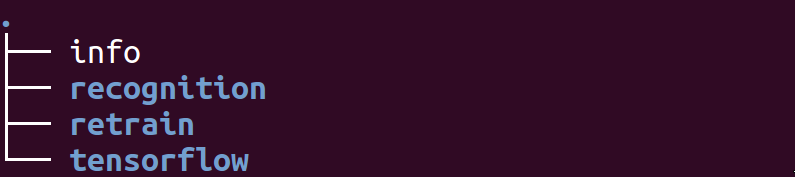
\includegraphics[width=\textwidth]{06.png}
	\caption{Verzeichnisstruktur Virtuelle Maschine}
	\label{fig:06}
\end{figure}

Alle benötigten Dateien befinden sich in dem \glqq{}retrain\grqq{}-Verzeichnis. In diesem Verzeichnis befindet sich einerseits das Python-Programm zum Retraining der neuen Klassen und ebenfalls die neu anzulernenden Klassen im \glqq{}images\grqq{}-Verzeichnis. Der Verzeichnisname beschreibt hierbei den Klassennamen und die darunterliegenden Dateien werden für das Retraining der Klasse verwendet.

\begin{figure}[!h]
	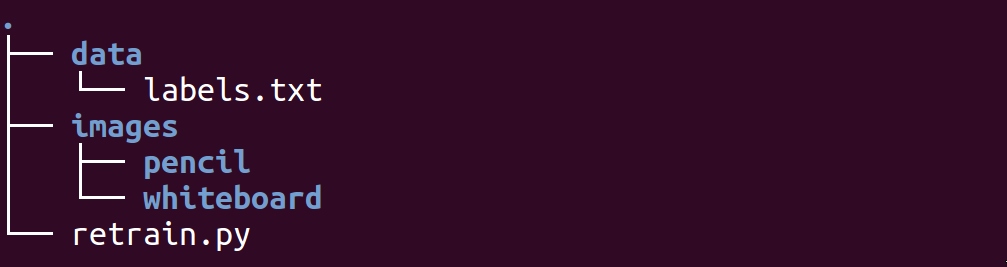
\includegraphics[width=\textwidth]{05.png}
	\caption{Verzeichnisstruktur \glqq{}retrain\grqq{}}
	\label{fig:05}
\end{figure}

\begin{figure}[!h]
	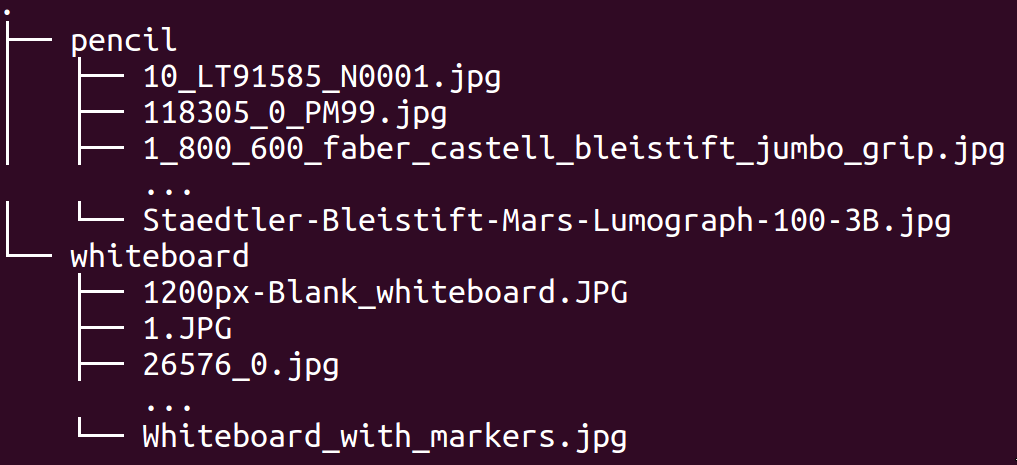
\includegraphics[width=\textwidth]{11.png}
	\caption{Verzeichnisstruktur der Klassen}
	\label{fig:11}
\end{figure}

Anschließend kann das Programm \glqq{}retrain.py\grqq{} mit dem folgenden Befehl ausgeführt werden.

\begin{lstlisting}[frame=single]
cd ~/tensorflow/retrain/
python retrain.py --image_dir=./images
\end{lstlisting}

Anschließend lädt das Programm das Inception V3 Modell herunter und führt das Retraining durch.

\begin{figure}[!h]
	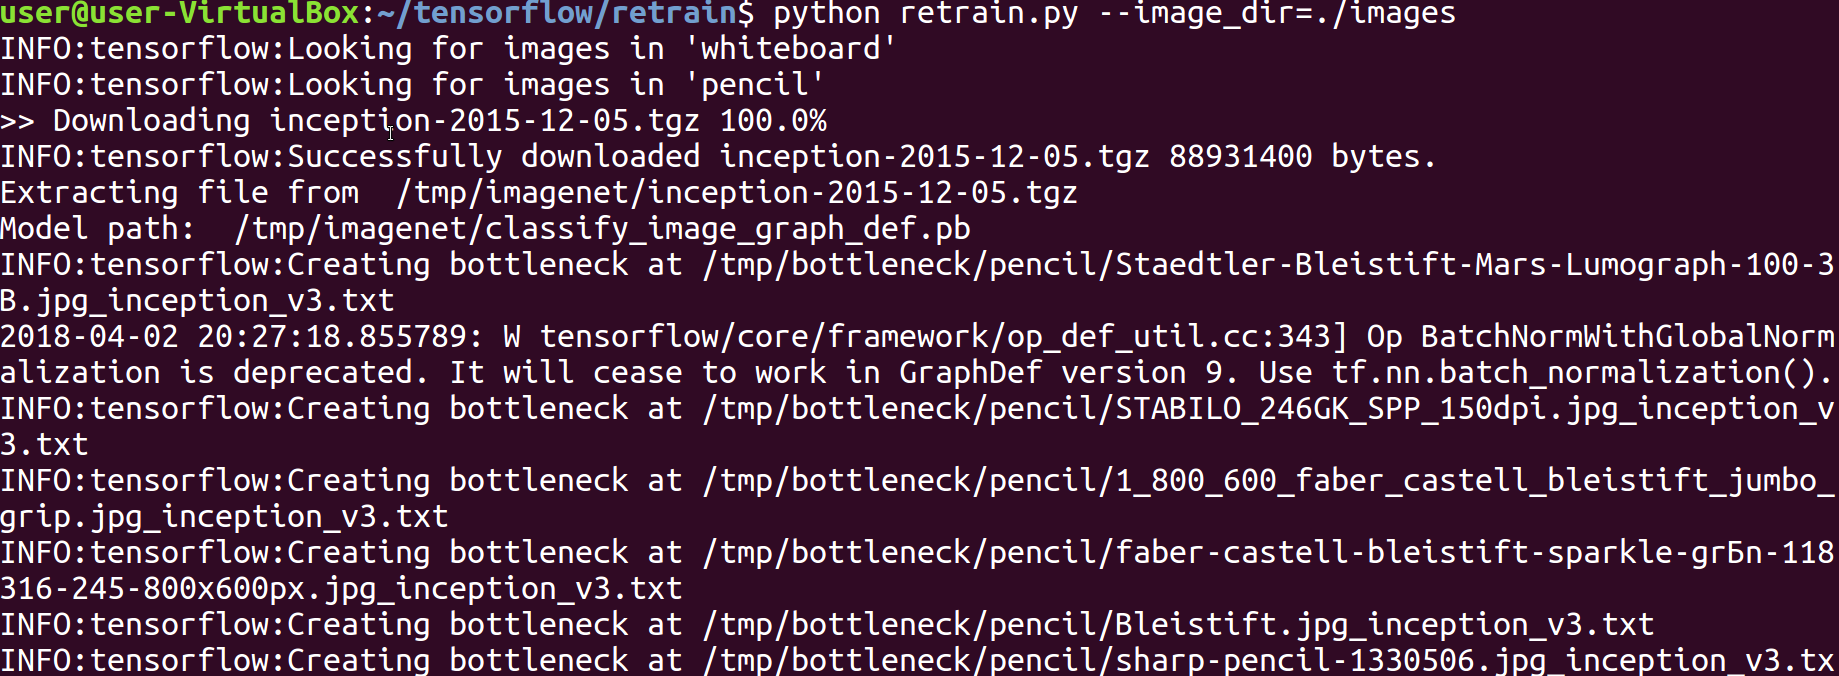
\includegraphics[width=\textwidth]{07.png}
	\caption{Retraining Konsolenausgaben: Bottleneck-Erstellung}
	\label{fig:07}
\end{figure}

Die Anwendung erstellt nun für jede vorhandene Datei eine sogenannte Bottleneckdatei. Hierbei handelt es sich um den vorfinalen Layer. Nachdem für jede Bilddatei eine Bottleneckdatei angelegt ist, wird das eigentliche Retraining durchgeführt. Die Ausgabe der Konsole sollte wie in Abbildung \ref{fig:08} dargestellt aussehen.

\begin{figure}[!h]
	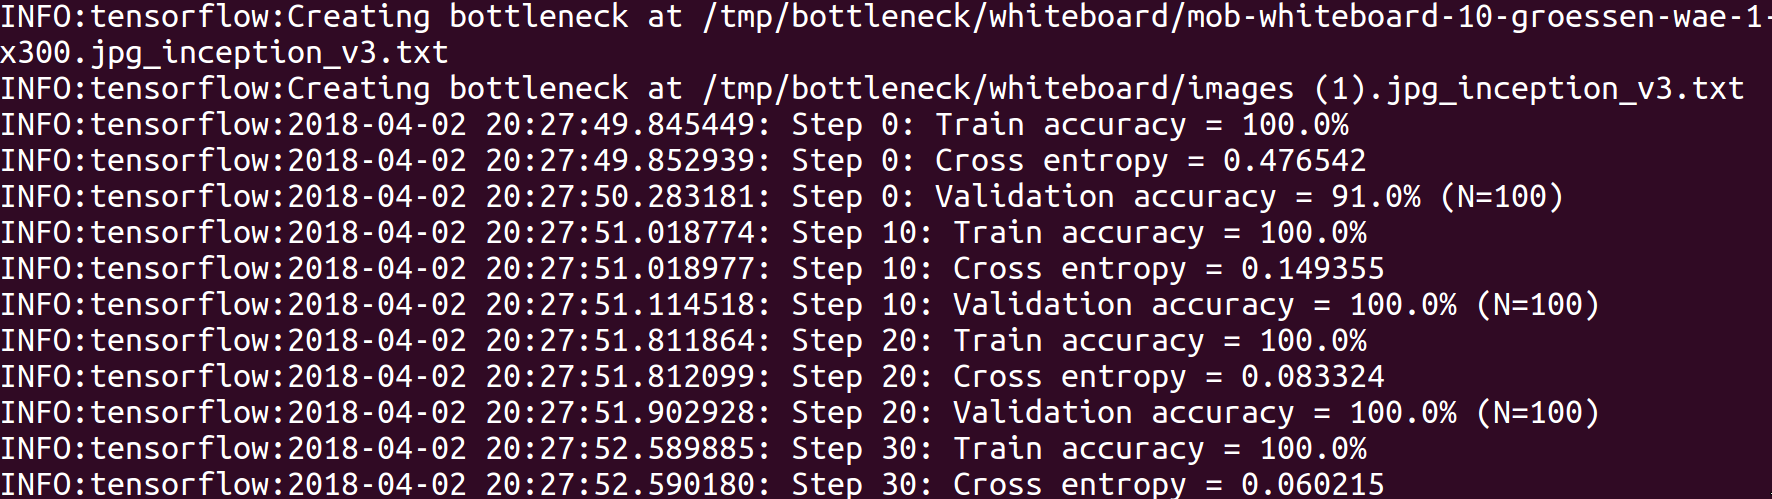
\includegraphics[width=\textwidth]{08.png}
	\caption{Retraining Konsolenausgaben: Retraining}
	\label{fig:08}
\end{figure}

Anschließend wird die Graph-Datei erstellt und die Bilderklassen wurden erfolgreich antrainiert.

\begin{figure}[!h]
	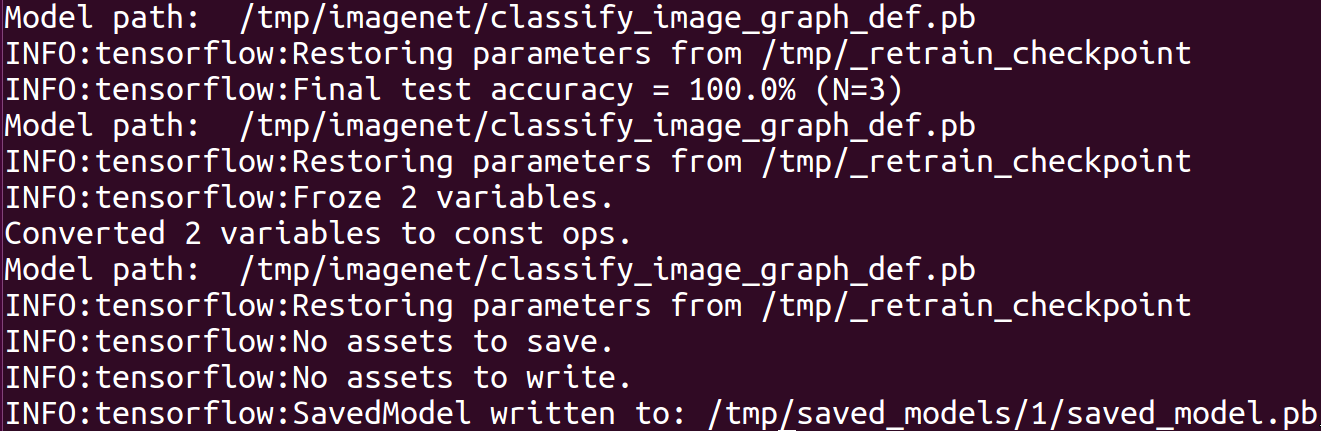
\includegraphics[width=\textwidth]{09.png}
	\caption{Retraining Konsolenausgaben: Graphdatei-Erstellung}
	\label{fig:09}
\end{figure}

\subsection{Image Recognition}
\label{subsec:trans-erstellung-mit-daten}
Nachdem die neuen Klassen antrainiert wurden, kann nun anschließend mit der Klassifizierung von Bildern begonnen werden. Hierfür werden die Dateien aus dem Verzeichnis \glqq{}recognition\grqq{} benötigt.

\begin{figure}[!h]
	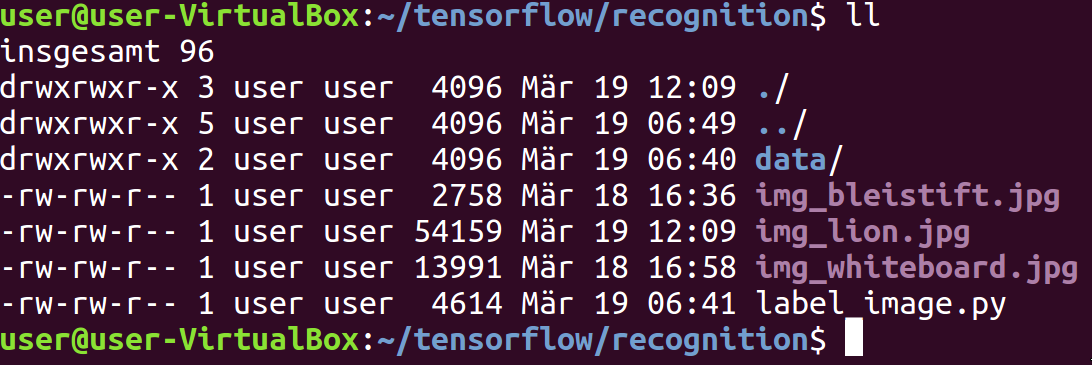
\includegraphics[width=\textwidth]{10.png}
	\caption{Recognition Verzeichnisstruktur}
	\label{fig:10}
\end{figure}

Um nun die neu trainierten Klassen zu verwenden müssen die Parameter bei Programmstart übergeben werden. Zunächst wird die vortrainierten Klassen getestet. Hierfür muss der folgende Befehl ausgeführt werden.

\begin{lstlisting}[frame=single]
cd ~/tensorflow/recognition/
python label_image.py --image=./img_whiteboard.jpg
\end{lstlisting}

Die Anwendung sollte das Bild des Whiteboards nicht erkennen, da die Whiteboard Klasse nicht in dem Inception V3 Modell vorhanden ist. Die Ausgabe sollte wie in Abbildung \ref{fig:12} dargestellt aussehen.

\begin{figure}[!h]
	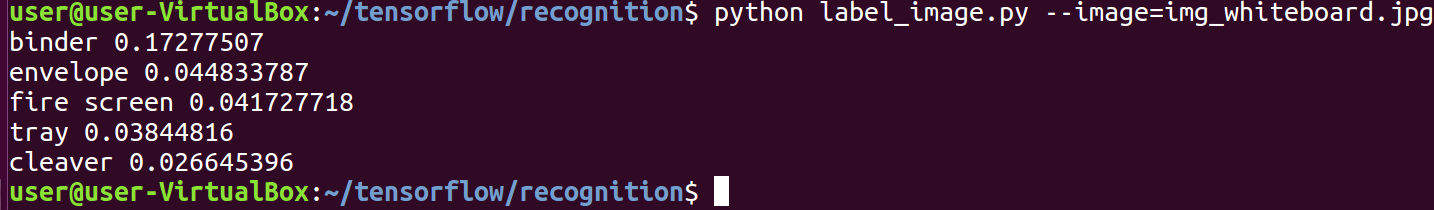
\includegraphics[width=\textwidth]{12.png}
	\caption{Recognition: Klasse nicht antrainiert}
	\label{fig:12}
\end{figure}

Anschließend wird mit dem folgenden Befehl ein Bild eines Löwen klassifiziert.

\begin{lstlisting}[frame=single]
cd ~/tensorflow/recognition/
python label_image.py --image=./img_lion.jpg
\end{lstlisting}

In diesem Beispiel sollte das neuronale Netz das Bild Klassifizieren können (Konsolenausgabe ist in Abbildung \ref{fig:13} dargestellt).

\begin{figure}[!h]
	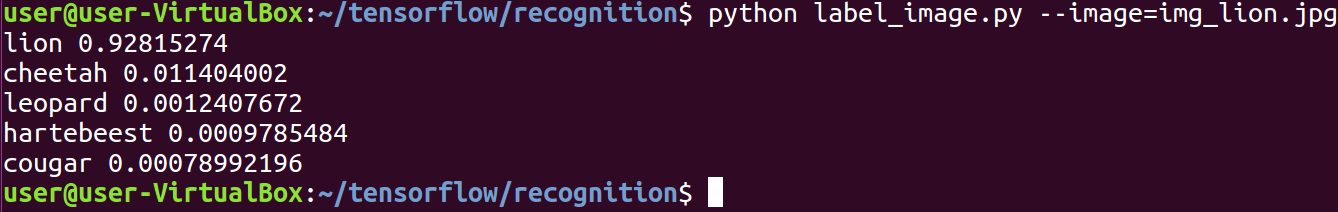
\includegraphics[width=\textwidth]{13.png}
	\caption{Recognition: Klasse antrainiert}
	\label{fig:13}
\end{figure}

Zuletzt wird das in Kapitel \ref{subsec:trans-erstellung} antrainierte Modell verwendet werden, sodass das Bild des Whiteboard erkannt werden kann. Hierfür müssen die Parameter der \glqq{}label\_image\grqq{}-Anwendung angepasst werden.

\begin{lstlisting}[frame=single]
cd ~/tensorflow/recognition/
python label_image.py --graph=/tmp/output_graph.pb --labels=output_labels --input_layer=Mul --output_layer=final_result --image=./img_whiteboard.jpg
\end{lstlisting}

Nachdem dieser Befehl ausgeführt ist, sollte die Konsole das Whiteboard klassifizieren können.

\begin{figure}[!h]
	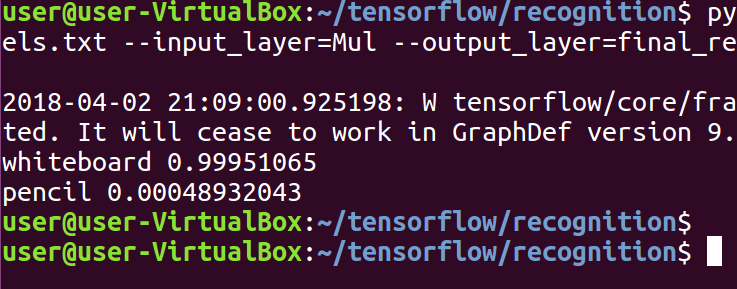
\includegraphics[width=\textwidth]{14.png}
	\caption{Recognition: Whiteboard erkannt}
	\label{fig:14}
\end{figure}

Der Parameter \glqq{}--graph\grqq{} steht für die Graph-Datei des trainierten neuronalen Netzwerks. Die Labels-Datei steht für die Klassen des Modells. Der Parameter \glqq{}--input\_layers\grqq{} definiert den Eingabe-Layer und \glqq{}--output\_layers\grqq{} den letzten Layer.

% !TEX root = ../document.tex
\section{Kritische Reflexion}
\label{sec:Kritik}
Es ist zu beachten, dass, auch wenn das Gebiet der Convolutional Neural Networks bereits 1989 erforscht wurde, hat das Thema der Bildverarbeitung erst in den letzten Jahren an großer Bedeutung gewonnen. Entsprechend ist das Thema sehr aktuell und wird momentan weiter erforscht, sodass die Literatur in diesem Themenbereich sich fortwährend ändert und somit die weitere Entwicklung beobachtet werden sollte. Des Weiteren ist anzumerken, dass die Funktionsweise des Convolutional Neural Networks, seiner Schichten und deren Mittel wie bspw. der Filter innerhalb dieser Arbeit nur oberflächlich dargestellt werden kann. So beruhen diese letztlich auf komplexen mathematischen Berechnungen, die bei Vertiefung dieses Themas betrachtet werden sollten. Außerdem ist zu erwähnen, dass das Convolutional Neural Network lediglich eine Variante zur Bildverarbeitung darstellt und hier als solche vorgestellt wird, da diese im vorgestellten Framework TensorFlow Verwendung findet.
% !TEX root = ../document.tex
\section{Fazit}
\label{sec:Fazit}
Letztlich lässt sich sagen, dass TensorFlow eine geeignete Möglichkeit für das Image Recognitioning darstellt. Die Verwendung fertiger Skripte macht eine schnelle Anwendung möglich und ist aufgrund der einfachen Verwendung auch schnell erlernbar. Durch die mitgelieferten Funktionen ist auch die eigene Entwicklung eines Convolutional Neural Networks problemlos möglich und dadurch, dass TensorFlow Open-Source ist, können auch bestehende Funktionen nach Belieben angepasst werden. TensorFlow macht es so möglich Machine Learning vor allem mit Hinblick auf Bildverarbeitung trotz komplexer mathematischer Theorie einfach verwenden zu können. Auch wenn das Convolutional Neural Network bereits eine sehr ausgereifte Art der Bildverarbeitung darstellt, wird dennoch weiterhin an neuen und effizienteren Methoden geforscht und auch versucht bestehende Möglichkeiten wie das Convolutional Neural Network stets weiterzuentwickeln, weshalb Interessierte sich in diesem sehr aktuellen Bereich des Image Recognitionings stets weiter informieren sollten.

	
	\clearpage
	\renewcommand{\refname}{Literaturverzeichnis}
	\bibliographystyle{plainnat}
	\bibliography{bibliography}
	
	\clearpage
	% !TEX root = document.tex

\section*{Eidesstattliche Erklärung}
\addcontentsline{toc}{section}{Eidesstattliche Erklärung}

Wir erklären an Eides statt, dass wir unsere Hausarbeit \\ \\
\glqq \titel \grqq{} \\ \\
selbstständig und ohne fremde Hilfe angefertigt haben und dass wir alle von anderen Autoren wörtlich übernommenen Stellen wie auch die sich an die Gedankengänge anderer Autoren eng anlehnenden Ausführungen unserer Arbeit besonders gekennzeichnet und die Quellen zitiert haben.
\\ \\

\begin{figure}[!h]
	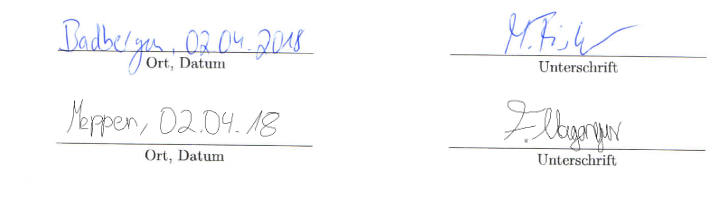
\includegraphics[width=\textwidth]{15.png}
\end{figure}
	
	\clearpage
	\appendix
	\pagenumbering{roman}
	% !TEX root = document.tex

% iwas.

	
\end{document}
